%! Author = louis
%! Date = 6/16/20
\documentclass[10pt,a4paper]{article}

\renewcommand{\familydefault}{\sfdefault}
\setlength{\parindent}{0pt}

\usepackage{../Summary}

\hyphenation{
	Kon-text-wech-sel
	Bub-ble-sort
	In-ser-tion-sort
	Merge-sort
	Count-ing-sort
}

\renewcommand{\lecture}{Algorithmen und Datenstrukturen}
\renewcommand{\student}{Louis Seubert}

\usepackage{enumitem}
\setlist[description]{style=nextline,noitemsep}
\setlist{nolistsep,noitemsep}

\usepackage{multicol}
\setlength{\columnseprule}{0.5pt}

\usepackage{color}
\usepackage{standalone}
\usepackage{tabularx}
\usepackage{changepage}

\usepackage{algorithmic}

\usepackage{tikz}
\usetikzlibrary{arrows,arrows.meta,automata,petri,trees,matrix,positioning}

\tikzstyle{b} = [circle, black, font=\bf\tt, draw=black, align=center, inner sep=0pt, text width=1.5em, text centered, very thick]
\tikzstyle{r} = [circle, red,   font=\bf\tt, draw=red,   align=center, inner sep=0pt, text width=1.5em, text centered, very thick]
\tikzstyle{n} = [rectangle, white, draw=black, align=center, inner sep=0pt, minimum width=0.5em, minimum height=0.5em]
\tikzstyle{o} = [circle, orange, draw=orange, align=center, inner sep=0.85em, very thick]
\tikzstyle{t} = [circle, teal,   draw=teal,   align=center, inner sep=0.85em, very thick]
\tikzstyle{h} = [blue, very thick]
\tikzstyle{n} = [black, thin]

% Document
\begin{document}
\begin{multicols*}{4}
\section{Allgemeines}
\subsection{Notationen}
\begin{center}
	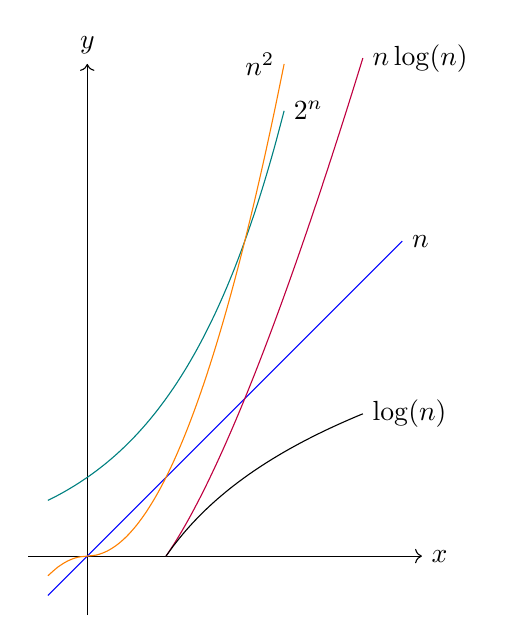
\begin{tikzpicture}
		\draw[->] (-0.75, 0) -- (4.25, 0) node[right] {$x$};
		\draw[->] (0, -0.75) -- (0, 6.25) node[above] {$y$};

		\draw[domain=-0.5:4,smooth,variable=\n,blue]
		plot ({\n},{\n}) node[right,black]{\(n\)};

		\draw[domain=-0.5:2.5,smooth,variable=\n,teal]
		plot ({\n},{2^\n}) node[right,black]{\(2^{n}\)};

		\draw[domain=-0.5:2.5,smooth,variable=\n,orange]
		plot ({\n},{\n^2}) node[left,black]{\(n^{2}\)};

		\draw[domain=1:3.5,smooth,variable=\n,purple]
		plot ({\n},{\n * log2(\n)}) node[right,black]{\(n \log(n)\)};

		\draw[domain=1:3.5,smooth,variable=\n]
		plot ({\n},{log2(\n)}) node[right,black]{\(\log(n)\)};
	\end{tikzpicture}
\end{center}

\subsubsection*{\OO-Notation}
Die \OO-Notation gibt eine \textbf{Obergrenze} einer Funktion an, unter berücksichtigung eines konstanten Faktors. Für
alle \(n\) welche größer sind als \(n_{0}\), ist Funktionswert der Funktion \(g(n)\) auf oder unter dem der Funktion
\(c \cdot f(n)\). Wir schreiben somit \(g(n) = \OO(f(n))\) um zu zeigen dass die Funktion \(g(n)\) ein Teil der Menge
\(\OO(f(n))\) ist.

\subsubsection*{\(\Omega\)-Notation}
Die \(\Omega\)-Notation gibt eine \textbf{Untergrenze} einer Funktion an, unter berücksichtigung eines konstanten
Faktors. Wie in Abbildung. Für alle \(n\) welche größer sind als \(n_{0}\), ist der Funktionswert der Funktion \(g(n)\)
auf oder über dem der Funktion \(c \cdot f(n)\). Wir schreiben somit \(g(n) = \Omega(f(n))\) um zu zeigen dass die
Funktion \(g(n)\) ein Teil der Menge \(\Omega(f(n))\) ist.

\subsubsection*{\(\Theta\)-Notation}
Die \(\Theta\)-Notation gibt eine \textbf{Obergrenze} sowie eine \textbf{Untergrenze} einer Funktion an , unter
berücksichtigung eines konstanten Faktors. (vgl. die letzten beiden Notationen)

\section{Sortieralgorithmen}
\begin{description}
	\item[Stabiler Sortieralgorithmus] Elemente mit zwei gleichen aufeinanderfolgenden Sortierschlüsseln bleiben im
	      sortierten Feld in der ursprünglichen Reihenfolge. \textit{Bsp:} Bubble Sort, Insertionsort, Merge Sort,
	      Counting Sort.
	\item[Eindeutigkeitsproblem] Algorithmus mit Laufzeit \(\OO(n)\)
	\item[Fibonaccizahl] Jeder bekannte Algorithmus mit ganzzahliger Arithmetik benötigt für die n-te Fibonaccizahl
	      immer mindestens \(\OO(n)\) viele Additionen
\end{description}

\subsection{Insertion Sort}
\subsubsection*{Herangehensweiße}
In einer Zahlenliste wird jedes Element einzeln an die richtige Stelle einfügt.
\subsubsection*{Vorgehensweise}
Es wird von links nach rechts, angefangen mit zweiten Element immer mit seinem Nachfolger verglichen, sollte der
Nachfolger ebenfalls kleiner sein als das Element, so wird der Vergleich mit dessen Nachfolger durchgeführt.
Sollte sich ein element finden welches größer ist so wird mit dem vermerkten Vorgänger getauscht.
\begin{align*}
	\tuple{42,63,12,85,17} & \quad\text{\small Vergleiche 63, 42, Korrekt} \\
	\tuple{42,63,12,85,17} & \quad\text{\small Vergleiche 12, 63, Tausche} \\
	\tuple{12,42,63,85,17} & \quad\text{\small Vergleiche 12, 42. Tausche}
\end{align*}
\subsubsection*{Laufzeitanalyse}
Im \textit{Idealfall} \(\OO(n)\), wenn die Liste bereits sortiert ist. Im \textit{Normalfall} \(\OO(n^{2})\).
Der \textit{Schlechtestefall} ist \(\sum_{i=1}^{n-1} i \in O(n^{2})\) wenn die Liste absteigend sortiert ist.
\subsubsection*{Implementierung}

\newcommand{\blockindent}{10}
\newcounter{indentation}
\newcommand{\keyword}[1]{{\bf#1}\;}


\newcommand{\foreachloop}[3]
{
	\keyword{foreach}#1\;\keyword{in}#2\;\keyword{do}
	\addtocounter{indentation}{\blockindent}
	{
		\begin{adjustwidth}{\value{indentation}pt}{}
			#3
		\end{adjustwidth}
	}
	\addtocounter{indentation}{-\blockindent}
}

\newcommand{\forloop}[3]
{
	\keyword{for}#1\;\keyword{to}#2\;\keyword{do}
	\addtocounter{indentation}{\blockindent}
	{
		\begin{adjustwidth}{\value{indentation}pt}{}
			#3
		\end{adjustwidth}
	}
	\addtocounter{indentation}{-\blockindent}
}

\newcommand{\whileloop}[2]
{
	\keyword{while}#1\;\keyword{do}
	\addtocounter{indentation}{\blockindent}
	{
		\begin{adjustwidth}{\value{indentation}pt}{}
			#2
		\end{adjustwidth}
	}
	\addtocounter{indentation}{-\blockindent}
}

\newcommand{\ifstat}[2]
{
	\keyword{if}#1\;\keyword{then}
	\addtocounter{indentation}{\blockindent}
	{
		\begin{adjustwidth}{\value{indentation}pt}{}
			#2
		\end{adjustwidth}
	}
	\addtocounter{indentation}{-\blockindent}
}

\newcommand{\ifelstat}[3]
{
	\keyword{if}#1\;\keyword{then}
	\addtocounter{indentation}{\blockindent}
	{
		\begin{adjustwidth}{\value{indentation}pt}{}
			#2
		\end{adjustwidth}
		\keyword{else}
		\begin{adjustwidth}{\value{indentation}pt}{}
			#3
		\end{adjustwidth}
	}
	\addtocounter{indentation}{-\blockindent}
}

\newcommand{\arrayat}[2]{#1{{\small[}\,{#2}\,{\small]}}}


\framebox{
	\begin{minipage}{0.93\linewidth}
		\textsc{InsertionSort}(A)\vspace{3px}\hfill\hline\hfill \\
		{\tt
		\forloop{i = 1}{Length(A)}
		{
			k = \arrayat{A}{j} \newline
			i = j - 1          \newline
			\whileloop{i > 0 and \arrayat{A}{i} > k}
			{
				\arrayat{A}{i + 1} = \arrayat{A}{i} \newline
				i = i - 1
			}
			\arrayat{A}{i + 1} = k
		}
		}
	\end{minipage}
}

\subsection{Selection Sort}
\subsubsection*{Herangehensweiße}
Das kleinstes Element des Feldes suchen und in einen Separaten Bereich schieben.
\subsubsection*{Vorgehensweise}
\begin{align*}
	\tuple{|42,63,12,85,17}       & \quad\text{\small 12 kleinste} \\
	\tuple{12 \,|\, 63,42,85,17}  & \quad\text{\small 17 kleinste} \\
	\tuple{12,17 \,|\, ,42,85,63} & \quad\text{\small 42 kleinste}
\end{align*}
\subsubsection*{Laufzeitanalyse}
In allen fällen beträgt die Laufzeit \(\Theta(n^{2})\)
\subsubsection*{Implementierung}
\framebox{
	\begin{minipage}{0.93\linewidth}
		\textsc{SelectionSort}(A)\vspace{3px}\hfill\hline\hfill \\
		{\tt
		\forloop{i = 1}{Length(A) - 1}
		{
			s = i \newline
			\forloop{j = i + 1}{Length(A)}
			{
				\ifstat{\arrayat{A}{j} < \arrayat{A}{s}}{
					s = j
				}
			}
			swap(\arrayat{A}{i},\arrayat{A}{s})
		}
		}
	\end{minipage}
}

\subsection{Merge Sort}
\subsubsection*{Herangehensweiße}
Teile das Feld bis nur noch ein einzelnes Elemente übrig ist im Anschluss vereinige diese dann jeweils sortiert.
\subsubsection*{Vorgehensweise}
\begin{align*}
	\tuple{42,63,12,85,17}                             & \quad\text{Verkleinere} \\
	\tuple{42}\tuple{63}\tuple{12}\tuple{85}\tuple{17} & \quad\text{Vereinige}   \\
	\tuple{42,63}\tuple{12,85}\tuple{17}               &                         \\
	\tuple{12,42,63,58}\tuple{17}
\end{align*}
\subsubsection*{Laufzeitanalyse}
In allen fällen beträgt die Laufzeit \(\Theta(n\log(n))\)
\subsubsection*{Implementierung}

\subsection{Bubble Sort}
\subsubsection*{Herangehensweiße}
\subsubsection*{Vorgehensweise}
\subsubsection*{Laufzeitanalyse}
\subsubsection*{Implementierung}

\subsection{Heap Sort}
\subsubsection*{Herangehensweiße}
Ein Feld wird als Binärbaum interpretiert, dabei muss zunächst die Max-Heap Eigenschaft hergestellt werden.
\subsubsection*{Vorgehensweise}
Um ein Feld zu sortieren muss zunächst die Max-Heap Eigenschaft hergestellt sein. Das bedeutet dass der Elternknoten
eines Knoten immer einen höheren Wert haben muss als er selbst.

Die Positionen im Feld lassen sich dabei wie folgt berechnen:
\begin{align*}
	\text{Elternknoten}(i)\quad       & \left\lfloor\frac{i}{2} \right\rfloor \\
	\text{Linker Kindknoten}(i) \quad & 2 \cdot i                             \\
	\text{Rechter Kindknoten}(i)\quad & (2 \cdot i) + 1
\end{align*}

\begin{center}
	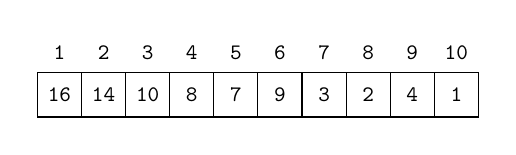
\begin{tikzpicture}
		[
			every node/.style={scale=0.8},
			font=\ttfamily,
			array/.style={
					matrix of nodes,
					nodes={draw, minimum size=7mm},
					column sep=-\pgflinewidth,
					row sep=0.5mm,
					nodes in empty cells,
					row 1/.style={nodes={draw=none, fill=none, minimum size=5mm}},
				}
		]
		\matrix[array,row 2 column 1/.style={fill=gray!30}] (array) {
			1  & 2  & 3  & 4 & 5 & 6 & 7 & 8 & 9 & 10                         \\
			16 & 14 & 10 & 8 & 7 & 9 & 3 & 2 & 4 & 1 \\};
	\end{tikzpicture}

	\begin{tikzpicture}
		[
			level distance=6.5mm,
			level 1/.style={sibling distance=32mm},
			level 2/.style={sibling distance=16mm},
			level 3/.style={sibling distance=8mm},
		]

		\node {16}
		child { node {14}
				child { node {8}
						child { node {2} }
						child { node {4} }
					}
				child { node {7}
						child { node {1} }
						child [missing]
					}
			}
		child { node {10}
				child { node {9} }
				child { node {3} }
			};
	\end{tikzpicture}
\end{center}

\subsubsection*{Laufzeitanalyse}

Das hat immer eine Laufzeit von \(\OO(n \log n)\).

\subsubsection*{Implementierung}

\framebox{
	\begin{minipage}{0.93\linewidth}
		\textsc{MaxHeapFix}(A,size,i)\vspace{3px}\hfill\hline\hfill \\
		{\tt
		l = Left(i)  \\
		r = Right(i) \\
		\ifelstat{l \(\leq\) size and \arrayat{A}{l} \(>\) \arrayat{A}{i}}
		{
			m = l
		}
		{
			m = i
		}
		\ifstat{r \(\leq\) size and \arrayat{A}{r} \(>\) \arrayat{A}{m}}
		{
			m = r
		}
		\ifstat{m \(\neq\) i}
		{
			swap(\arrayat{A}{i},\arrayat{A}{m}) \\
			MaxHeapFix(A, size, m)
		}
		}
	\end{minipage}
}

\framebox{
	\begin{minipage}{0.93\linewidth}
		\textsc{HeapSort}(A)\vspace{3px}\hfill\hline\hfill \\
		{\tt
		size = a.length \\
		\forloop{i = \(\floor{\text{size} \div 2}\)}{\(1\)}
		{
			MaxHeapFix(A,size,i)
		}
		\forloop{i = size}{\(2\)}
		{
			swap(\arrayat{A}{1},\arrayat{A}{i}) \\
			size = size - 1                     \\
			MaxHeapFix(A,size,1)
		}
		}
	\end{minipage}
}

\subsection{Quick Sort}
\subsubsection*{Herangehensweiße}
\subsubsection*{Vorgehensweise}
\subsubsection*{Laufzeitanalyse}
\subsubsection*{Implementierung}

\subsection{Counting Sort}
\subsubsection*{Herangehensweiße}
Halte ein zusätzliches Feld welches die Anzahl der Vorkommenden Zahlen speichert und dann im Anschluss in das
ursprüngliche Feld der Reihe nach einfügt.
\subsubsection*{Vorgehensweise}
\begin{align*}
	\tuple{5,4,3,1,4,1,1} & \quad C = \tuple{3,0,1,2,1} \\
	\tuple{1,1,1,?,?,?,?} & \quad C = \tuple{0,0,1,2,1} \\
	\tuple{1,1,1,3,?,?,?} & \quad C = \tuple{0,0,0,2,1} \\
	\tuple{1,1,1,3,4,4,?} & \quad C = \tuple{0,0,0,0,1}
\end{align*}
\subsubsection*{Laufzeitanalyse}
In allen fällen beträgt die Laufzeit \(\OO(n+k)\) wobei \(k\) die Anzahl der möglichen Werte im Feld ist.
\subsubsection*{Implementierung}
Der Parameter \textit{max} entspricht dem maximalen Wert welcher in dem Feld vorkommen kann. \hfill

\framebox{
	\begin{minipage}{0.93\linewidth}
		\textsc{CountingSort}(A,max)\vspace{3px}\hfill\hline\hfill \\
		{\tt
		C = new [0..max] \\
		\foreachloop{i}{A}
		{
			\arrayat{C}{i} = \arrayat{C}{i} + 1
		}
		\forloop{i = 1}{max}
		{
			\arrayat{C}{i} = \arrayat{C}{i} + \arrayat{C}{i - 1}
		}
		B = new [1..max] \\
		\forloop{i = A.length}{1}
		{
			v = \arrayat{A}{i} \\
			\arrayat{B}{\arrayat{C}{v}} = v \\
			\arrayat{C}{v} = \arrayat{C}{v} - 1
		}
		}
	\end{minipage}
}

\subsection{Radix Sort}
\subsubsection*{Herangehensweiße}
Die Elemente welche sortiert werden, haben der annahme nach alle die gleiche Länge. So wird dann die Sortieren immer auf
eine Stelle der Elementenschlüssels begrenzt und mit einem stabilen Verfahren sortiert.
\subsubsection*{Vorgehensweise}
Alle Elementenschlüssel werden in Einzelschlüssel unterteilt und beginnend mit dem am wenigsten signifikaten Schlüssel
sortiert.

(Zeichenketten z.b. Basis: 26)
\subsubsection*{Laufzeitanalyse}
In allen fällen beträgt die Laufzeit \(\OO(w \cdot n)\) wobei \(w\) der Anzahl der Einzelschlüsseln entspricht.
\subsubsection*{Implementierung}
Ist abhängig von dem verwendeten Verfahren.

\section{Bäume}

\subsection{Binäre Suchbäume}
Jeder Knoten hat einen linken und einen rechten Kindknoten. Jeder Konten besitz einen Schlüssel, in dem rechte
Teilbaum sind die Schlüssel der Knoten größer als der Schlüssel der Wurzel. In dem linken Teilbaum sind die
Schlüssel der Knoten kleiner als der Schlüssel der Wurzel. Teilbäume sind auch ebenfalls wieder Binärbäume,
\emph{für die die gleiche Eigenschaft rekursiv mit deren Knotenwert gilt}.

Bei einer optimalen Belegung (jeder Knoten hat zwei Kindknoten) hat ein Baum mit \(n\) Ebenen insgesamt
\(2^{n+1} - 1\) Konten. Dabei hat dieser auf der Ebene \(n\), \(2^{n}\) Knoten.

\subsubsection{Anzahl möglicher Suchbäume}
Bei einer Anzahl von \(n\) Knoten gibt es \(C_{n}\) möglichkeiten mit
\[C_{n} = \cfrac{1}{n+1} \cdot \binom{2n}{n} = \cfrac{(2n)!}{(n+1)! \cdot n!}\]

\subsubsection{Einfügen}
Begonnen wird bei der Wurzel, der Schlüssel wird verglichen ist dieser größer wird in den rechten Teilbaum weiter
verfahren, ansonsten wird in den linken Teilbaum weiterverfahren. Sollte ein \NIL Knoten gefunden werden,
dann wird das Element diesen 'Knoten' ersetzen. \\

\framebox{
	\begin{minipage}{0.93\linewidth}
		\textsc{Insert}(r, n)\vspace{3px}\hfill\hline\hfill \\
		{\tt
		y = null \\
		x = r    \\
		\whileloop{x \(\neq\) null}{
			y = x \\
			\ifelstat{n.key \(<\) x.key}
			{
				x = x.left
			}
			{
				x = x.right
			}
		}
		n.parent = y \\
		\ifelstat{y \(=\) null}
		{
			r = n
		}
		{
			\ifelstat{n.key \(<\) y.key}
			{
				y.left = v
			}
			{
				y.right = v
			}
		}
		}
	\end{minipage}
}

\subsubsection{Suchen}
Das Verfahren ist ähnlich zu dem des Einfügens nur das bei einem Vergleich auch die Gleichheit von den Schlüsseln
mit berücksichtigt wird. Sollten diese gleich sein ist das Element gefunden worden. Die Laufzeit dafür beträgt
\(\log n\). Sollte ein \NIL 'Knoten' zuvor erreicht werden so ist das Element nicht im Baum vorhanden. \\

\framebox{
	\begin{minipage}{0.93\linewidth}
		\textsc{Search}(x, k) \vspace{3px}\hfill\hline\hfill \\
		{\tt
		\ifstat{x = null or k = x.key}
		{
			\keyword{return} x
		}
		\ifstat{k \(<\) x.key}
		{
			\keyword{return} search(x.left, k)
		}
		\keyword{return} search(x.right, k)
		}
	\end{minipage}
}

\subsubsection{Minimum und Maximum}
Das Minimum und Maximum zu finden ist bei einem Suchbaum welcher sortiert ist einfach: Das \textbf{kleinste} Element
ist das am \textbf{linkesten} und das \textbf{größte} Element das was am \textbf{rechtesten} im Baum zu finden ist.

\subsubsection{Nachfolger}

\framebox{
	\begin{minipage}{0.93\linewidth}
		\textsc{Successor}(x) \vspace{3px}\hfill\hline\hfill \\
		{\tt
		\ifstat{x.right = null}
		{
			\keyword{return} min(x.right)
		}
		p = x.parent\\
		\ifstat{p != nil and p.right = x}
		{
			x = p \\
			p = p.parent
		}
		\keyword{return} p
		}
	\end{minipage}
}

\subsubsection{Löschen}
Bei dem löschen eines Knoten gibt es drei mögliche Szenarien:
\begin{enumerate}
	\item Der zu löschende Knoten besitzt \textbf{kein} Kindknoten, in diesem Fall kann der Knoten einfach gelöscht
	      werden.
	\item Der zu löschende Knoten besitzt \textbf{einen} Kindknoten, in diesem Fall wird der zu löschende einfach
	      mit seinem Kindknoten überschrieben.
	\item Der zu löschende Knoten besitzt \textbf{zwei} Kindknoten, in diesem Fall kann einer der Nachfolger
	      aufrücken und dessen Platzt einnehmen.
\end{enumerate}

\subsubsection{Traversierung}
\begin{description}
	\item[Pre Order] Wurzel, Links, Rechts
	\item[In Order] Links, Wurzel, Rechts \\
	      Gibt die Sortierreihenfolge an
	\item[Post Order] Links, Rechts, Wurzel
\end{description}

\subsection{Rot-Schwarz-Bäume}
\textcolor{red}{\sc Wichtig}\hfill\\
In der Klausur darf kein \textcolor{red}{Rot} benutzt werden!

\subsubsection{Eingenschaften}
\begin{enumerate}
	\item Knoten haben immer eine Farbe, sie können entweder ROT oder SCHWARZ sein
	\item Die Wurzel eines Baumes ist immer SCHWARZ
	\item Jedes Blatt eines Baumes (\NIL) ist immer SCHWARZ
	\item Ist ein Knoten ROT, dann sind seine beiden Kinder immer SCHWARZ \\
	      Somit können nie zwei rote Knoten nacheinander kommen
	\item Die Anzahl der SCHWARZEN Knoten auf dem Weg zu einem nachfolgenden \NIL 'Knoten' ist geht immer durch die
	      gleiche Anzahl an SCHWARZEN Knoten
\end{enumerate}

\begingroup
\newcommand{\inc}[1]{\includestandalone[scale=0.8]{#1}}
\newcommand{\uncle}{\textcolor{orange}{Onkel}\;}

\newcommand{\rnode}[1]{\raisebox{-.6ex}{\tikz{\node[scale=0.65, font=\bfseries\footnotesize, r]{#1};}}\,}
\newcommand{\bnode}[1]{\raisebox{-.6ex}{\tikz{\node[scale=0.65, font=\bfseries\footnotesize, b]{#1};}}\,}

\subsubsection{Einfügen}
Zunächst verhält sich das Einfügen wie in einem regulären Binärbaum.

Ein neuer Knoten \rnode{Z} ist zunächst immer Rot, um die Schwarzhöhe konstant zu halten. Ansonsten wird wie folgt
vorgegangen:

\begin{table}[H]
	\centering
	\begin{tabular}{l|c|c}
		\textbf{Fall} & Eingefügt               & Fix                     \\ \hline
		1.            & \rnode{Z}               & \bnode{Z}               \\ \hline
		\multicolumn{3}{c}{ \rnode{Z}\texttt{.parent} ist rot und}        \\ \hline
		2.            & \inc{assets/01-rb-tree} & \inc{assets/02-rb-tree} \\ \hline
		              & \inc{assets/03-rb-tree} & \inc{assets/04-rb-tree} \\
		3.            & \inc{assets/05-rb-tree} & \inc{assets/06-rb-tree} \\ \hline
		              & \inc{assets/07-rb-tree} & \inc{assets/08-rb-tree} \\
		4.            & \inc{assets/09-rb-tree} & \inc{assets/10-rb-tree} \\ \hline
	\end{tabular}
\end{table}

Beachte das in dem Beispiel die \NIL Knoten weggelassen worden sind.

\begin{enumerate}
	\item Das Element ist die Wurzel
	\item Der \uncle von \rnode{Z} ist ebenfalls \textsc{rot} \(\rightarrow\) \\
	      Umfärben der Ebenen von \mbox{\rnode{Z}.\texttt{parent}} bis \mbox{\rnode{Z}.\texttt{parent}.\texttt{parent}}.
	      Sollte die \textbf{Wurzel} ebenfalls \textsc{rot} sein, dann \textit{Regel 1}
	\item Der \uncle von \rnode{Z} ist \textsc{schwarz} \(\rightarrow\) \\
	      \mbox{\rnode{Z}.\texttt{parent}} in die entgegengesetzte Richtung zu rotieren, so dass \rnode{Z} an dessen
	      Stelle steht. Erzeugt die Regel 4.
	\item Der \uncle von \rnode{Z} ist \textsc{schwarz} \(\rightarrow\) \\
	      \mbox{\rnode{Z}.\texttt{parent}.\texttt{parent}} und \mbox{\rnode{Z}.\texttt{parent}} werden umgefärbt, dann
	      ersteren in die entgegengesetzte Richtung rotieren, so dass \mbox{\rnode{Z}.\texttt{parent}} an dessen Stelle
	      steht.
\end{enumerate}

\endgroup

\subsection{B-Bäume}
B-Bäume sind oftmals benutzt für die Zugriffsminimierung bei externen Speichermedien. Knoten heißen in einem B-Baum
Seiten und haben eine gewisse Anzahl \(n\).

\begin{figure}[H]
	\centering
	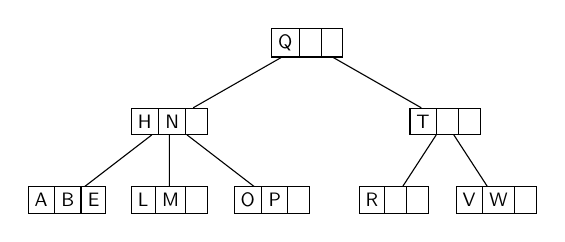
\begin{tikzpicture}
		\tikzstyle{every node}=[scale=0.7, rectangle split, rectangle split horizontal, rectangle split parts = 3, draw]

		\tikzstyle{level 1}=[sibling distance=35mm, level distance=10mm]
		\tikzstyle{level 2}=[sibling distance=13mm, level distance=10mm]

		\node {Q}
		child {
				node  {H \nodepart{two} N}
				child {node {A\nodepart{two} B\nodepart{three} E}}
				child {node {L\nodepart{two} M}}
				child {node {O\nodepart{two} P}}
			}
		child {
				node {T}
				child {node {R}}
				child {node {V \nodepart{two} W}}
			}
		;
	\end{tikzpicture}
\end{figure}

\subsubsection{Eigenschaften}
\begin{enumerate}
	\item Ein Knoten hat maximal \(m\) Kindknoten
	\item Ein Knoten (ohne Wurzelknoten) hat minimal \(\ceil{m\div2}\) Kindknoten
	\item Der Wurzelknoten hat mindestens 2 Kindknoten, wenn er selbst kein Blattknoten ist
	\item Ein Knoten mit \(k\) Kindknoten besitzt \(k-1\) Schlüssel
	\item Der \textbf{Baumgrad} eines Baumes legt somit fest: \\
	      \textbf{Die Mindestanzahl an Schlüsseln pro Knoten} (ohne Wurzelknoten): \(t-1\) \\
	      \textbf{Die Maximalanzahl an Schlüsseln pro Knoten}: \(2t-1\)
\end{enumerate}

\subsubsection{Bedingungen}


\paragraph*{Baumhöhe}\hfill\\
Die minmale Höhe des Baumes mit \(n\) Knoten ist \(h_{\text{min}} = \ceil{\log_{m}(n+1)} - 1\)

Die maximal Höhe des Baumes mit \(n\) Knoten ist \(\floor{\log_{d}((n+1) \div 2)}\)

\subsubsection{Einfügen}
Zunächst verhält sich das Einfügen wie in einem regulären Binärbaum.

Nach dem finden des Knoten in den das Element eingefügt werden soll, wird dieses sortiert in diesen Konten eingefügt,
nun muss die Anzahl der Elemente in diesem Knoten überprüft werden:
\begin{enumerate}
	\item Sollte der Knoten weniger als die maximale Anzahl an zugelassenen Elementen, muss nichts weiter getan werden.
	\item Ist der Knoten nun an seiner maximalen Anzahl angekommen bzw. hat diese überschritten so muss der Knoten
	      aufgeteilt werden:
	      \begin{enumerate}
		      \item Ein Mittelwert wird gewält aus allen Elementen in dem Knoten
		      \item Elemente welche kleiner sind als der gewählte Mittelwert sind nun Elemente eines neuen Knotens
		            welcher nun der \textit{linke} Kindknoten des Mittelwertes ist
		      \item Elemente welche größer sind al der gewählte Mittelwert sind nun Elemente eines neuen Knotens welcher
		            nun der \textit{rechte} Kindknoten des Mittelwertes ist
	      \end{enumerate}
\end{enumerate}

\section{Hashverfahren}

\subsection{Hashfunktionen}

\subsubsection{Divisionsmethode}
Dabei wird eine Zahl \(k\) modulo \(m\) gerechnet, dieser vorgang wird dann als das eigentliche Hashing bezeichnet.
Idealerweise ist \(m\) eine Primzahl welche nicht in der nähe einer Potenz von zwei ist. \[h(k) = k \bmod m\]

\subsubsection{Multiplikationsmethode}
\[h(k) = \floor{m \cdot \underbrace{\left((k \cdot A) \bmod 1\right)}_\text{Nachkommastellen}}\]
Ein Vorschlag für ein solches A von Donald Kunth: \(A = \cfrac{\sqrt{5}-1}{2} \approx 0,618033\)

\subsection{Kollisionsauflösung}

\subsubsection{Geschlossene Addressierung}
Der Schlüsselindex steht fest, sollte es zu einer Kollision kommen dann wird das neue Element in einem getrennten
Bereich eingefügt. Dieser Bereich kann so etwas wie eine einfach verkettete Liste sein.

Der \textbf{Belegungsfaktor} \(\alpha =\frac{n}{m}\) setzt sich zusammen aus der größe der Hash Tabelle \(m\) und der Anzahl
der Zellen im Primärbereich \(n\).

Die Anzahl der Vergleiche bzw. Zugriffe bei einer erfolgreichen bzw. erfolglosen Suche ist im Mittel:
\(\Theta(1+\alpha)\)

Sollte die Anzahl der Slots proportion sein zur Anzahl der Elemente in der Tabelle so ist die Suche im Mittel in
konstanterzeit durchzuführen. Somit sind alle Operationen im Mittel mit \(\OO(1)\).

\subsubsection{Offene Addressierung}
Alle Elemente werden in der Hash Tabelle gespeichert. Jedes Element wird einem \emph{Slot} zugeordnet, das suchen nach
einen solchen Slot wird dann \textbf{sondieren} genant. Dabei gibt es noch einen weiteren Parameter die sogenannte
\textbf{Sondierungszahl}.

Bei einem Löschen aus einer solchen Hash Tabelle, kann kein null Wert gespeichert werden, somit git es ein neues Element
welches als Entfernt gilt.

\subsubsection*{Lineares Sondieren}
Bei linearen Sondieren werden alle Werte nacheinander (Laufindex \(i = 0,1,2,\dots,m-1\)) nach einem freien Platz
durchsucht \[h(k,i) = (h'(k) + i) \bmod m\]

Problematisch ist dabei die bildung von langen Clusterfolgen bei vielen gleichen Schlüsseln.

\subsubsection*{Quadratisches Sondieren}
Ist analog zum linearen Sondieren, lediglich die Hashfunktion ist mit zwei weiteren Konstanten versehen.
\[h(k,i) = (h'(k) + c_{1} \cdot i + c_{2} \cdot i^{2}) \bmod m\]

Problematisch ist dabei das nicht immer alle Indices in betracht kommen wenn die länge des Hash Tabelle ungeschickt ist.
Eine geschickte Wahl wäre \(3 \bmod 4\), da so alle Indices produziert werden.

\subsubsection*{Doppel-Hashing}
Ist analog zum linearen Sondieren, lediglich zwei hilfs Hashfunktionen werden verwendet.
\[h(k,i) = \left(h_{1}(k) + i \cdot h_{2}(k)\right) \bmod m\]

Zu beachten ist dabei das \(h_{2}(k) \neq 0\)

\section{Gierige Algorithmen}

Ein gieriger Algorithmus kann ein Problem lösen welches aus mehreren einzel Problemen besteht welche überlappen.

\subsection{Entwurfsschemata}

\subsubsection*{Indirekter Ansatz}
\begin{enumerate}
	\item Bestimme optimale Teilproblem-Struktur
	\item Entwickle eine rekursive Lösung
	\item Zeige, dass bei einer \emph{gierigen} Wahl nur ein Teilproblem verbleibt
	\item Zeige, dass die \emph{gierige} Wahl korrekt ist
	\item Entwickle rekursiven Algorithmus für die \emph{gierige} Strategie
	\item Wandle den rekursiven Algorithmus in einen iterativen um
\end{enumerate}

\subsubsection*{Direkter Ansatz}

\subsection{Aktivitäten Auswahl Problem}

\paragraph{Problem}
Liste von Aktivitäten mit Start- und Endzeiten müssen für einen bestimmten Zeitraum möglichst effizient, dass bedeutet
möglichst viele ohne Überschneidungen, in den Zeitraum untergebracht werden.

\paragraph{Lösungsansatz}
Wähle die Aktivität \(a_{1}\), die als erstes fertig ist, dadurch ist noch am meisten Zeit für die anderen Aktivitäten.

\textbf{Beweis:} Sei \(a_{1}\) nun \(a_{j}\) mit einem späteren Endzeitpunkt. Da nun die Resource exklusiv zugeteilt
wird dürfen sich niemals Aktivitäten überschneiden, somit kann bei der Wahl von \(a_{j}\) statt \(a_{1}\) die Anzahl
der freien Zeitslots entweder gleichbleiben oder sinken. Somit könnte eine andere optimale Lösung existieren, diese
hätte aber nie mehr Elemente als dieLösungsmenge mit der gierigen Wahl.

\paragraph{Teilproblem}
Das Finden der Aktivität welche nach dem Ende von \(a_{1}\) beginnt.

\textbf{Beweis:} \(a_{1}.\mathtt{start} < a_{1}.\mathtt{end}\) und \(a_{1}.\mathtt{end}\) ist der früheste Zeitpunkt.
Alle mit \(a_{1}\) verträglichen Aktivitäten müssen also später beginnen.

\section{Graphentheorie}

Ein Graph wird definiert mit \(G = (V,E)\), wobei \(V\) der Knotenmenge entspricht und \(E\) der Kantenmenge.

Die Übergangsfunktion kann mittels einer Adjazenzliste dargestellt werden, dabei wird von einem Knoten ausgehend alle
erreichbaren Knoten angegeben (Platzbedarf: \(\Theta(\abs{V}+\abs{E})\)). \(A \rightarrow B,D\) (Von \(A\) ist \(B,D\) erreichbar)

Neben der Adjazenzliste gibt es auch noch die Adjazenzmatrix, welche die Übergangsfunktion in einer \(p \times p\)
Matrix darstellt (Platzbedarf: \(\Theta(\abs{V}^2)\)).

\subsection{Ebene Graphen}

Ein ebener Graph ist ein Graph welcher ohne Überschneidungen von Kanten gezeichnet werden kann.

\subsubsection*{Symmetrischer Graph}

Ein symmetrischer Graph ist ein Graph welche keine gerichteten Kanten besitzt.

\subsection{Zusammenhangskomponente}

\textit{Beachte:}\hfill\\
Ein \textbf{zulässiger} Weg beachtet in einem Graphen die Richtung der Kanten.

\subsubsection*{Starke Zusammenhangskomponente}
Je zwei Knoten sind über einen \textbf{zulässigen} Weg miteinander verbunden. Dabei ist darauf zu achten das von jedem
Knoten jeder andere Knoten erreicht werden kann. (Wenn von \(A \rightarrow B\) dann muss auch \(B  \rightarrow A\)
vorkommen, somit entsteht ein Zyklus)

\subsubsection*{Schwache Zusammenhangskomponente}
Je zwei Knoten sind über einen \textbf{zulässigen} oder auch \textbf{nicht zulässigen} Weg miteinander verbunden.

\subsubsection*{Zweifache Zusammenhangskomponente}

\subsection{Suchen im Graphen}

\subsubsection*{Breitensuche - BFS}
Traversiere den Graphen beginnend von einem Knoten zunächst zu allen Nachfolgern dieses Knoten, sind alle besucht, so
besuche nun alle Nachfolger der Nachfolger. Das Prinzip wiederholt sich bis alle Knoten besucht worden sind.
Laufzeit: \(\OO(\abs{V}+\abs{E})\)

\subsubsection*{Tiefensuche - DFS}
Traversiere den Graphen beginnend von einem Knoten immer zu einem Nachfolger, solange bis kein Nachfolger mehr existiert
welcher nicht schon bekannt ist. Ist kein Nachfolger mehr verfügbar so geht man eine "Ebene" nach oben.
Laufzeit: \(\OO(\abs{V}+\abs{E})\)

\subsubsection*{Kürzester Weg - Dijkstra}
Beginne mit einem Knoten \(A\) und bilder ein Tuple \((A,A,0)\), wobei \((\texttt{Nach},\texttt{Von},\texttt{Gewicht})\)
entspricht.

Nun Bilde die selben Tuple für alle Verbindungen welche von Knoten \(A\) ausgehen. Wähle im Anschluss das Tuple aus
welches das kleinste Gewicht hat. Die anderen Tuple bleiben dabei unverändert als Auswahlmöglichkeiten.

Wiederhohle das nun das ganze solange bis die Auswahlmöglichkeiten erschöpft sind. Dabei ist zu beachten das falls ein
Knoten bereits schon einmal als Ziel auftritt überprüft werden muss ob die bestehende Verbindung kürzer ist, sollte das
der Fall sein so wird einfach weiter gemacht, wenn nicht wird diese ersetzt.

\begin{figure}[H]
	\centering
	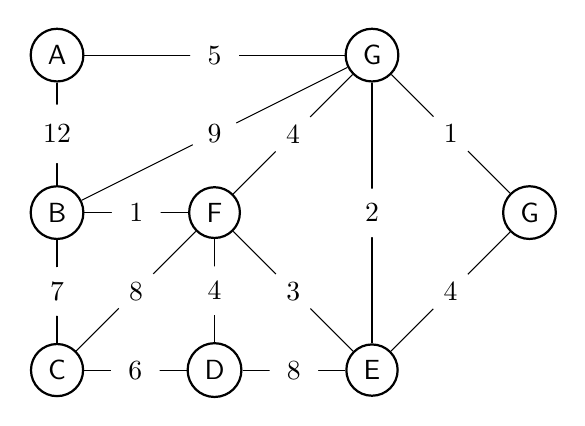
\begin{tikzpicture}
		\begin{scope}[every node/.style={circle,thick,draw}]
			\node (A) at (0,4) {A};
			\node (B) at (0,2) {B};
			\node (C) at (0,0) {C};

			\node (D) at (2,0) {D};
			\node (F) at (2,2) {F};

			\node (E) at (4,0) {E};
			\node (G) at (4,4) {G};
			\node (H) at (6,2) {G};
		\end{scope}

		\begin{scope}[every node/.style={fill=white,circle}]
			\path (A) edge node {$12$} (B);
			\path (A) edge node {$5$} (G);
			\path (B) edge node {$9$} (G);
			\path (B) edge node {$7$} (C);
			\path (B) edge node {$1$} (F);
			\path (C) edge node {$6$} (D);
			\path (C) edge node {$8$} (F);
			\path (D) edge node {$8$} (E);
			\path (F) edge node {$3$} (E);
			\path (F) edge node {$4$} (D);
			\path (F) edge node {$4$} (G);
			\path (E) edge node {$4$} (H);
			\path (G) edge node {$2$} (E);
			\path (H) edge node {$1$} (G);
		\end{scope}
	\end{tikzpicture}
\end{figure}

\begin{table}[H]
	\tt\footnotesize
	\centering
	\begin{tabular}{l|l}
		(A,A, 0) & (G,A, 5); (B,A,12)            \\
		(G,A, 5) & (B,A,12); (F,G, 9); (E,G, 7); \\
		(H,G, 6) & (B,A,12); (F,G, 9); (E,G, 7)  \\
		(E,G, 7) & (B,A,12); (F,G, 9); (D,E,15)  \\
		(F,G, 9) & (B,A,12); (D,E,15); (C,F,17)  \\
		(B,A,12) & (D,E,15); (C,F,17)            \\
		(D,E,15) & (C,F,17)                      \\
		(C,F,17) & \(\varnothing\)
	\end{tabular}
\end{table}

\subsection{Gewichtete Graphen}

\subsubsection*{Algorithmus von Prim}
Berechnung des Minimal Spanning Trees mit hilfe eines \emph{gierigen Algorithmus}. Dabei wird immer der Knoten mit dem
kleinsten Kantengewicht gewählt.

\subsubsection*{Algorithmus von Kruskal}
Berechnung des Minimal Spanning Trees mit hilfe eines \emph{gierigen Algorithmus} in einem \emph{ungerichteten Graphen}.
Dabei werden die Kanten der Größe nach sortiert und in eine Kopie des Graphen ohne Kanten eingefügt. Sollte dabei eine
Kante auftreten welche zwei bereits verknüpfte Knoten verbindet, so wird diese \textbf{ignoriert}.

\section{Korrektheitsbeweise}

\subsubsection*{Vorgehen}
\begin{enumerate}
	\item Initialisierung, setzte die Laufvariable \(i\) auf den Startwert.
	\item Zeige das die allgemeine Aussage vor beginn korrekt ist.
	\item Fortsetzung, setzte \(i'=i\) mit einer Schranke für \(i\)
	\item Setze \(i'\) in die Invariante ein und beweise das die darausfolgenden Ausdrücke korrekt sind (wenn z.b. die
	      Behauptung der Invariante genutzt wird)
	\item Terminierung, einsetzen der Laufvariable eins über dem maximum.
\end{enumerate}

Wichtig ist es:
\begin{itemize}
	\item Verschachtelte Schleifen müssen separat betrachtet werden
	\item Fallunterscheidungen mittels if müssen separat betrachtet werden
\end{itemize}

\subsection*{Beispiel}

\begin{algorithmic}[h]
	\STATE {\textsc{SUMME}(A,s,e)}
	\STATE{summe = 0}
	\FOR {i = s \TO e}
	\STATE {summe = summe + A[i\(i\)]}
	\ENDFOR
\end{algorithmic}

\[\text{summe}=\sum_{k=s}^{i-1}A[k]\]

\subsubsection*{Initialisierung}
\[\text{summe} = \sum_{k=s}^{s-1}A[k] = 0\]
Ist korrekt da noch keine Operation durchgeführt wurde und die summe null sein soll.

\subsubsection*{Fortsetzung}
\(i' = i \quad\wedge\quad s \leq i \leq e \)

\[\text{summe} = \sum_{k=s}^{i'-1}A[k]\]
dann im Algorithmus mit:
\[\text{summe} = \sum_{k=s}^{i'-1}A[k]+A[i'] = \sum_{k=s}^{i'}A[k]\]
nun gilt \(i=i'+1\) somit folgt \(i'=i-1\). Nun einsetzen und die gesamt aussage ist korrekt.

\subsubsection*{Terminierung}
\(i > e \implies i = e + 1\)
\[\text{summe} = \sum_{k=s}^{e+1-1}A[k] = \sum_{k=s}^{e}A[k]\]

\section{Amortisierte Analyse}
Mit der amortisierten Analyse bestimmt man die durchschnittliche benötigte Zeit für alle Operationen über einer
gegebenen Sequenz bzw. Datenstruktur. Dabei benötigen einige Operationen weniger Zeit als andere Operation.

Dabei unterscheidet sich die amortisierte Analyse von der durchschnittlichen Laufzeit darin das bei der
durchschnittlichen Laufzeit nur eine möglicher Wert heraus kommt. Hingegen bei der amortisierten Analyse wird
eine garantierte durchschnittliche Zeit für jede Operation im schlechtesten Fall zurück gegeben.

Dabei kann nach drei Unterschiedlichen vorgehensweiße vorgegangen werden:
\begin{itemize}
	\item Aggregations Analyse
	\item Konto Methode (Accounting)
	\item Potenzial Methode (Potential)
\end{itemize}

\end{multicols*}
\end{document}